\documentclass[12pt]{article}
\usepackage{amsfonts, epsfig}
\usepackage[authoryear]{natbib}
\usepackage{graphicx}
\usepackage{fancyhdr}
\pagestyle{fancy}
\lfoot{\texttt{comsm0021.github.io}}
\lhead{Neural Information Processing - 5\_Eriksen\_flanker - Conor}
\rhead{\thepage}
\cfoot{}
\begin{document}

\section*{Sensory processing: the Eriksen flanker task}

In this section we will talk about another experiment providing
evidence for Bayesian inference in the brain. In this case we will
start off examine our ability to pick out an individual in a crowd\footnote{A still from Hitchcock's film \textsl{Strangers on a Train}.}
\begin{center}
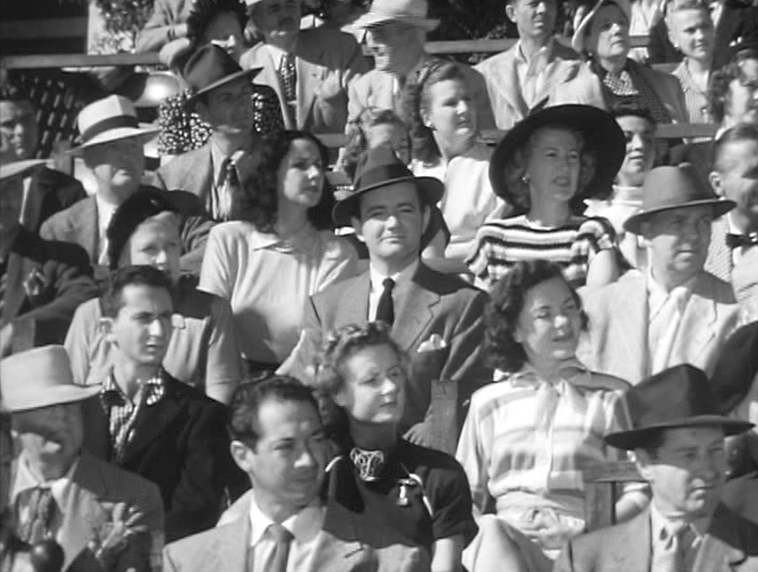
\includegraphics[width=7.5cm]{Strangers_on_a_Train.png}
\end{center}
though in the end we appear to observe something else. In any case we
begin by thinking about the selective attention and monitoring of
contrast and similarity in visual input. In the task the participants
are shown one of two stimuli, here a \lq{}\textbf{S}\rq{} or a
\lq{}\textbf{H}\rq{} and they press a button in reponse, for example
left for \textbf{S} and right for \textbf{H}. The target letter is
flanked by distractors on each side the participants are told to
ignore. There are two cases, one where the distractors are compatible:
\textbf{HHHHH} and \textbf{SSSSS} and one where they are incompatible:
\textbf{HHSHH} and \textbf{SSHSS}.

Participants are slower and less accurate when responding to
incompatible flankers. This is studied from a Bayesian point of view
in \cite{YuDayanCohen2009}; they use data from older experiments in
which the participants were instructed to perform the task as quickly
as possible. One surprising result, see Fig.~\ref{fig_rt_accurate}, is
that for very short reaction times the response with incompatible
flankers can be worse than chance.

\begin{figure}[tb]
\begin{center}
  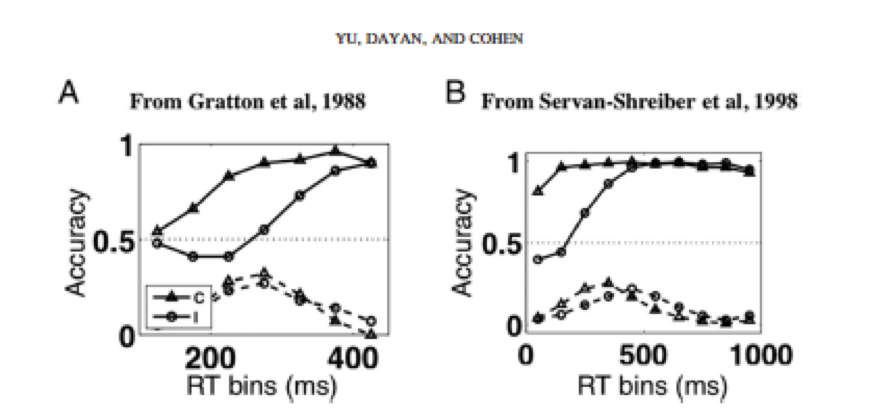
\includegraphics[width=9.5cm]{fig_rt_accurate.png}
\end{center}
\caption{The solid lines show the accuracy against reaction
  time; the dashed lines the distribution of reaction times themselves. There are two traces, one marked C with compatible flankers, this is graphed with triangles and one marked I with incompatible flankers. The figure was taken (by Rosalyn) from \cite{YuDayanCohen2009} but they themselves have adopted it from other studies. \label{fig_rt_accurate}}
\end{figure}
\bibliographystyle{apa}
\bibliography{../../source/bibliography}{}

There are two hypothises as to what is going on, the first is that
there is a compatibility bias: the brain assumes that the world is
smooth, so having \textbf{S} flankers biases it towards the
expectation that middle letter is also a \textbf{S}. This makes sense,
visual information often has a high regularity. 

The second hypothesis argues that the areas of the brain that perform
high level recognition assess visual stimuli over a large receptive
field and so the recognition neurons are receiving cross talk from the
distractors.

To see if these hypotheses account for the phenomenon we will
construct a \textsl{generative model}, that is a model that could
produce fictive data with a presumed similar distribution to the real
data. Here, the generative model is a model of a neuronal response to
the stimuli. We will couple the generative model to a
\textsl{recognition model}, a model of how the brain might identify
the target, based on the information encoded in the neurons. The
recognition model describes the decision and ultimately determines
which button will be pressed. 

Let the stimuli be labels $s_1$, $s_2$ and $s_3$, $s_2$ is the target,
$s_1$ are the letter to the left and $s_3$ to the right. In the
experiment $s_1=s_3$, in the compatible condition $s_1=s_2$, in the
incompatible $s_1\not=s_2$. The three neurons corresponding to three
stimuli are labelled $x_1$, $x_2$ and $x_3$; these will have a
response which is different, on average, depending on which letter is
in each part of the stimulus, but they will respond in a variable
way. In fact, for definiteness, lets say the $i$th stimulus $s_i=-1$
when the letter is \textbf{S} and $s_i=1$ if it is \textbf{H}; the
$x_I$ are then Gaussian distibuted around these values. Of course, in
line with hypothesis two, each neuron will get an input from more than
one $s_i$. The random variable $M$ describes the trial condition, with
$M=I$ for incompatible and $M=C$ for compatible. If $\mu_i=\mu(s_i)$
represented the zero or one at the $i$ subinterval in the hot house
then we have
\begin{equation}
p(\textbf{})
\end{equation}








\end{document}

